\documentclass[conference]{IEEEtran}
\IEEEoverridecommandlockouts
% The preceding line is only needed to identify funding in the first footnote. If that is unneeded, please comment it out.
\usepackage{cite}
\usepackage{amsmath,amssymb,amsfonts}
\usepackage{algorithmic}
\usepackage{graphicx}
\usepackage{textcomp}
\usepackage{xcolor}
\def\BibTeX{{\rm B\kern-.05em{\sc i\kern-.025em b}\kern-.08em
    T\kern-.1667em\lower.7ex\hbox{E}\kern-.125emX}}
\begin{document}

\title{Wall following Reactive Robot in ROS}

\author{\IEEEauthorblockN{Ana Barros}
\IEEEauthorblockA{\textit{M.EIC} \\
\textit{FEUP}\\
Porto, Portugal \\
up201806593@fe.up.pt}
\and
\IEEEauthorblockN{Henrique Melo Ribeiro}
\IEEEauthorblockA{\textit{M.EIC} \\
\textit{FEUP}\\
Porto, Portugal \\
up201806529@up.pt}
\and
\IEEEauthorblockN{João Costa}
\IEEEauthorblockA{\textit{M.EIC} \\
\textit{FEUP}\\
Porto, Portugal \\
up201806560@fe.up.pt}

}

\maketitle

\begin{abstract}

In this article, we will describe an implementation of a reactive robot with the objective of following walls. The terrain that forms the map has the shape of a \textit{squarer} C-cedilla ("Ç") letter, and the robot should stop when it reached the bottom of the cedilla. To simulate these conditions, the flatland simulator for ROS was used, using a modeled turtle bot. To locate itself, the robot uses LIDAR, which is a method to determine ranges using the time a laser targeted at an object or surface takes to return to the robot.

\end{abstract}

\begin{IEEEkeywords}
ROS, reactive robot, wall-following, LIDAR, flatland, simulation
\end{IEEEkeywords}

\section{Introduction}

The recent trend for robot autonomy calls for greater intelligence in these robots. One of the most interesting aspects of this \textit{intelligence} is its ability to emerge from simple behavior.

This article will focus on the simulation of a purely reactive robot with no memory developed to follow the walls of a given map, or to search for them in case they are not detected. The job is made harder by the limited capabilities of the robot: no state storage (no memory), no prior knowledge of the map, and no information regarding the current global position. In other words, the robot can only decide based on the current information gathered by the sensors.

We implemented the robot in the \emph{Flatland}\footnote{https://flatland-simulator.readthedocs.io/en/latest} simulator for \emph{ROS}\footnote{https://www.ros.org}. This environment allows for lightweight 2D physics simulations. The simulated robot is based on the \emph{TurtleBot 3}\footnote{https://www.turtlebot.com} and will use LIDAR to \textit{see the world}.

\section{State of the art}

Typically, wall-following algorithms fall under the \textbf{bug algorithms} umbrella. As stated by Howie Choset, these algorithms assume only local knowledge (e.g., follow a wall (right or left)) to reach a destination \cite{choset_robotic_nodate}. In contrast to the situation described in those slides, our robot does not have a way to measure its current distance to the goal. It can only identify the goal when it reaches it.

Karl Bayer suggests an expression ``\eqref{bayerEq}'' to calculate the angular velocity, $\omega$, of a robot following a wall to its left that depends on the distance and angle of the robot to the wall, the minimum distance to keep from the wall, and on the wall's curvature \cite{bayer_wall_nodate}.

\begin{equation}
\omega = (-k(sin(q_3) - (q_2 - T) + K) v \label{bayerEq}
\end{equation}

Mingxin Liu further builds on this equation, adding corrections for the length of the robot, and accounting for sensors in different positions providing different readings (i.e., different parts of the robot can be at different distances from the wall) \cite{liu_comparison_2020}.

It should be noted that the approaches described benefit from keeping state, either with (PID) controllers or otherwise, which is something that we cannot do.

\section{The task}

\subsection{Controlling the robot}

The robot has a control for the linear velocity and one for the angular velocity. By default, the simulated robot doesn't have limits on these velocities, and they don't take into consideration any \textit{realistic} maximum acceleration value.

In order to have a more \textit{realistic} simulation and perform experiments with different values, we limited the maximum velocity and acceleration of the robot (to configurable values).

\subsection{The map}

A mentioned previously, the map (in ``Fig.~\ref{fig:map}'') is shaped like a \textit{squarer} C-cedilla ("Ç") letter.

\begin{figure}[htbp]
    \centerline{
\includegraphics{images/c.png}}
    \caption{The simulation map (spawn area highlighted in red).}
    \label{fig:map}
\end{figure}

At the start of the simulation, the robot spawns somewhere inside the curved part of the map with a random orientation.

\subsection{Locating the first wall}

Once placed on the map, the robot will perform a random walk (referred to as \emph{wiggle}) until finding a wall. In order to prevent long periods of circling in place, we reset (to zero) the angular velocity of the robot when it reaches the maximum when \emph{wiggling}.

\subsection{The sensors}

The robot has a LiDAR sensor that performs measurements in 270º (from -135º to 135º) around it, in intervals of 2.5º. This leads to 108 measurements 10 times per second, i.e., one scan every 100 milliseconds. The measurements performed by the sensor has an artificial error leading to a standard deviation of 0.1. Each measurement of a scan reports the angle (relative to the front of the robot) and the distance to the detected obstacle. The maximum range of the sensors is 3 meters.

When reaching a scan, the robot divides the measurements into 8 regions (``Fig.~\ref{fig:lidar}''): front, front\_left, left, back\_left, back, back\_right, right, and front\_right. It should be noted that since the sensors do not cover the full 360º around the robot, there are no measurements for the back regions and for parts of the back\_left and back\_right regions.

\begin{figure}[htbp]
    \centerline{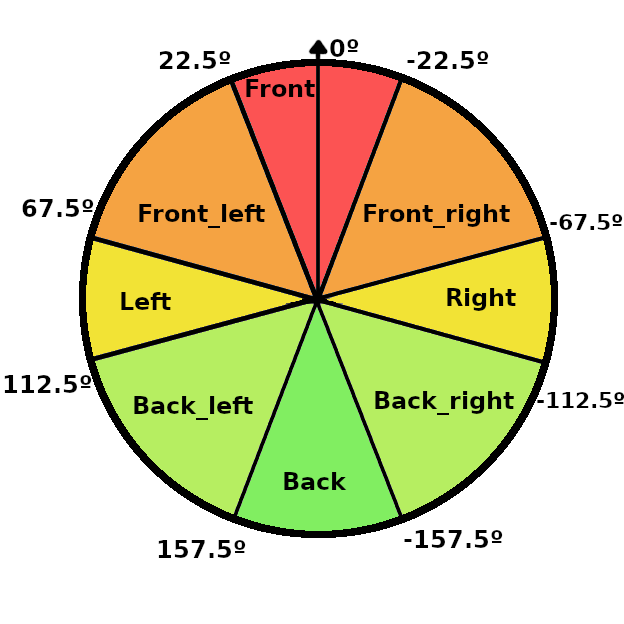
\includegraphics{images/lidar.png}}
    \caption{The 8 regions of a LiDAR scan.}
    \label{fig:lidar}
\end{figure}

\subsection{Following the wall}

The robot's reaction to the scan depends on several factors: the direction it is currently facing (in relation to the wall), which side is closest to the wall, and the distance to the surrounding walls.

First, the linear velocity of the robot is inversely proportional to the distance to the closest obstacle in front of the robot (i.e., the closer the obstacle is, the lower the linear velocity). This helps the robot react to corners without crashing into the wall in front of it.

After setting the linear velocity, the robot then needs to adjust the angular velocity. The robot Karl Bayer describes on his paper can only follow walls on its left side. We wanted our robot to be able to follow walls on either side. The direction the turtle bot will rotate depends on which side is closest to a wall. On top of that, depending on if the robot is closer to the wall than it should be (its distance to the wall is smaller than the minimal distance allowed), the robot will rotate in the opposite direction to correct this. This leads to a movement patter similar to ``Fig.~\ref{fig:robot_movement}''.

\begin{figure}[htbp]
    \centerline{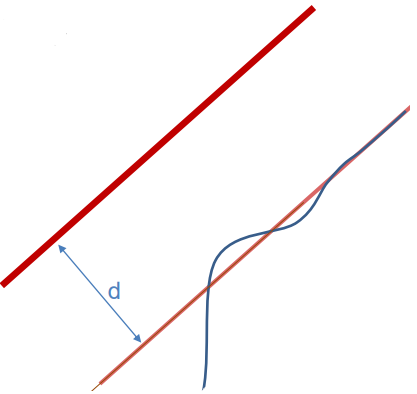
\includegraphics[width=0.5\linewidth]{images/robot_movement.png}}
    \caption{Approximation of the movement of the robot (blue line) \cite{locomotion}}
    \label{fig:robot_movement}
\end{figure}

As stated previously, our sensor's measurement angle is relative to the front of the robot. We can estimate the direction of the robot in relation to the closest wall using the ray that measured the shortest distance. By assuming that the shortest ray hits the wall at approximately 90º, we can calculate the direction of the robot relatively to the wall as $\frac{\pi}{2} - rayDirection$ ``Fig.~\ref{fig:wall_angle}''.

\begin{figure}[htbp]
    \centerline{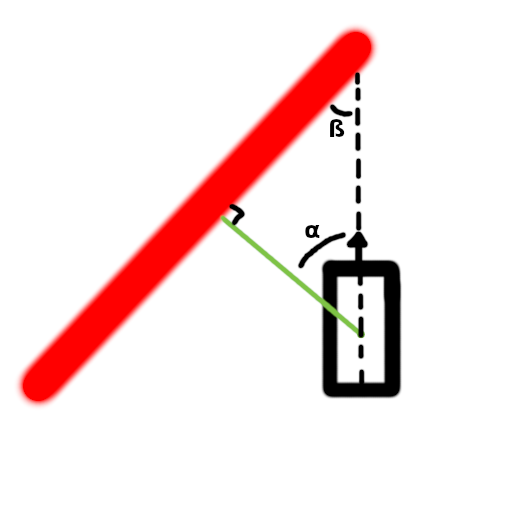
\includegraphics{images/wall_angle.png}}
    \caption{Rationale behind the robot direction estimation.}
    \label{fig:wall_angle}
\end{figure}

With this, we end up with two equations, adapted from ``\eqref{bayerEq}'', ``\eqref{leftEq}'' and ``\eqref{rightEq}'' for following a wall to left and to the right respectively. Notice that we do not use the wall curvature parameter, $K$, since the author did not seem of its usefulness and the calculation is difficult.

When the robot approaches a wall while following a wall, e.g., when approaching the cedilla, the front of the robot will become the part that is closest to a wall (see ``Fig.~\ref{fig:corner}). However, if the robot were to use the method previously described, it would likely turn around following the wall it was following until that point. To solve this, we implement a check for obstacles in front of the robot. When the robot detects an obstacle ahead while following a wall, it turns away from the wall sidewall that it was following. After rotating enough to stop detecting the obstacle ahead, it will continue applying the usual algorithm to follow the new wall; the obstacle that triggered this situation.

\begin{figure}[htbp]
    \centerline{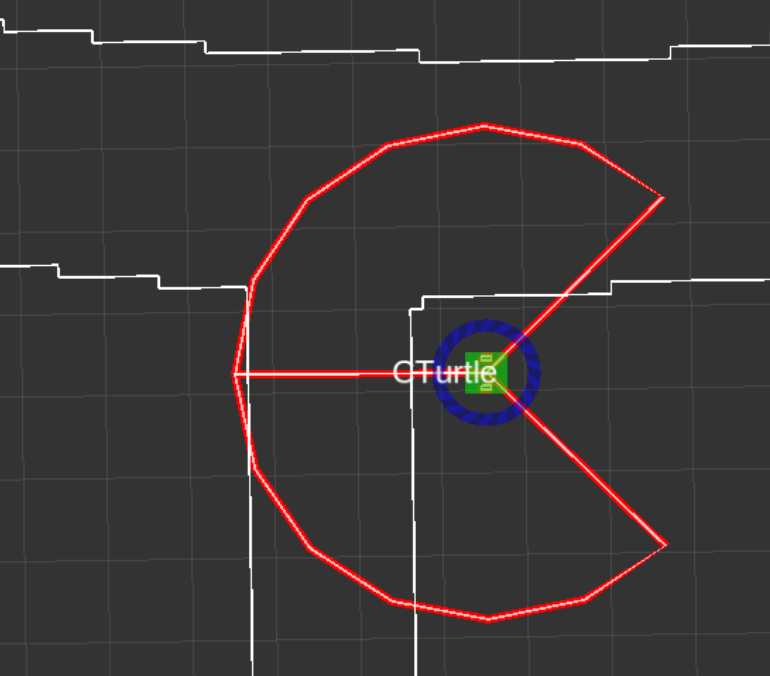
\includegraphics[width=0.5\linewidth]{images/corner.png}}
    \caption{The robot approaching a corner.}
    \label{fig:corner}
\end{figure}

\begin{equation}
\omega = (-k(cos(q_3) - (q_2 - T)) v \label{leftEq}
\end{equation}

\begin{equation}
\omega = (-k(cos(pi - q_3) - (q_2 - T)) v \label{rightEq}
\end{equation}

\subsection{Stopping at target location}

The goal of the robot is to follow the walls until reaching the desired destination. This destination is the lowest part of the map, i.e., the bottom of the cedilla of the C letter. This proved to be challenging, as the C part of the letter contained two different regions that resembled the cedilla: the edges of the curved parts.

The main difference of those two regions and the cedilla is the size (length) of the flat surface. Taking this into account, the safest approach to detect if the robot is at the cedilla or not is to calculate the length of the wall.

In order to be able to calculate said distance some pre-processing must be done, which is, turning the LiDAR measures from distance and angle into coordinates relative to the robot (i.e., the robot is at the origin of the coordinate system). This point-cloud is obtained through ``\eqref{eq:coords}'', where $L$ is the length of the laser and $\alpha$ is the angle of the laser. To calculate the length of the wall, the robot sums the distance between each pair of points of the wall. The flat bottom part of cedilla measures around 2 meters in the simulation. The robot checks if the detected length is within a $10\%$ margin of this value.

\begin{equation}
coords = (L * cos(\alpha), L * sin(\alpha)) \label{eq:coords}
\end{equation}

This calculation revealed to be insufficient, as during some turns and moments when the robot was first approaching a wall, the measured length would equal the length of the cedilla. This was caused by the limited range of the sensors. There's an additional check to prevent these false positive: verifying if the right or left (depending on which side of the robot is closest to the wall) back laser collide with a wall (``Fig.~\ref{fig:stop_region}''). In case the laser does not collide with any wall, the robot checks the length of the wall in order to determine if it is at bottom of the cedilla. 

When the robot detects the bottom of the cedilla, it breaks in order to stop at the intended spot. However, since the robot is purely reactive, high values of linear velocity coupled with low braking power can lead to problems stopping at right location; the robot might not be able to halt in time. The robot has no memory/state to record the fact that it has reached the end/target region, so it needs to be detecting this region for as long as it takes to brake. As such, it is important to increase the breaking power of the robot when increasing its maximum linear velocity, to prevent it from never stopping.

\begin{figure}[htbp]
    \centerline{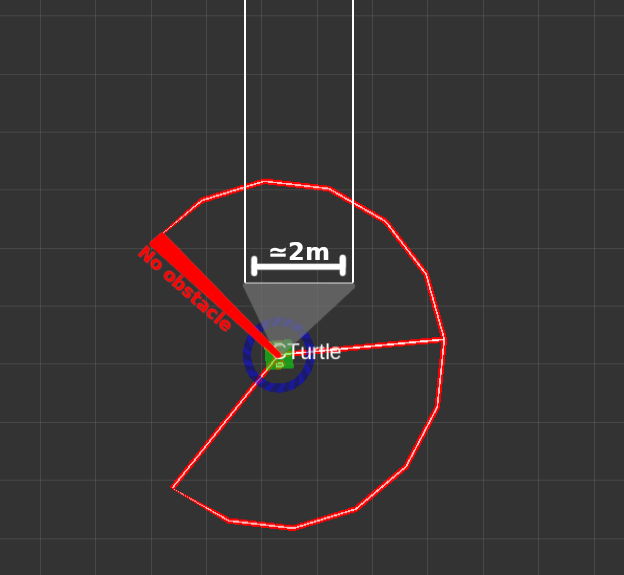
\includegraphics{images/stop_region.png}}
    \caption{Robot detecting the stop region.}
    \label{fig:stop_region}
\end{figure}

\section{Experiments and results}
\label{sec:results}

``Tab.~\ref{tab:experiments}'' contains experiments performed with the final version of the robot. Each row represents a new experiment with different values. The \textit{Time} column represents the time it took the robot to finish a lap around the map. The \textit{Direction} column indicates on which side the robot followed the wall (right or left). The rest of the columns depict the values for the angular and linear acceleration, deceleration, and maximum velocity for each experiment. ``Fig.~\ref{fig:path}'' plots the robot path for each experiment using the ground truth provided by the simulator.

\begin{table*}[htbp]
\caption{Loop time experiment results}
\begin{center}
\begin{tabular}{|c|c|c|c|c|c|c|c|c|}
\hline
\textbf{Number} & \textbf{\begin{tabular}[c]{@{}c@{}}Time \\ ($s$)\end{tabular}} & \textbf{Direction} & \textbf{\begin{tabular}[c]{@{}c@{}}Ang. Accel. \\ ($rad/s^2$)\end{tabular}} & \textbf{\begin{tabular}[c]{@{}c@{}}Ang. Decel \\ ($rad/s^2$)\end{tabular}} & \textbf{\begin{tabular}[c]{@{}c@{}}Max. Ang. vel. \\ ($rad/s$)\end{tabular}} & \textbf{\begin{tabular}[c]{@{}c@{}}Lin. accel. \\ ($m/s^2$)\end{tabular}} & \textbf{\begin{tabular}[c]{@{}c@{}}Lin. decel. \\ ($m/s^2$)\end{tabular}} & \textbf{\begin{tabular}[c]{@{}c@{}}Max. lin. vel.\\ ($m/s$)\end{tabular}} \\ \hline
1 & 93.27 & left & 4.0 & 4.0 & 3.0 & 1.5 & 3.0 & 2.0 \\ \hline
2 & 85.37 & left & 8.0 & 8.0 & 3.0 & 1.5 & 3.0 & 2.0 \\ \hline
3 & 58.25 & left & 20.0 & 20.0 & 3.0 & 2.0 & 3.0 & 3.0 \\ \hline
4 & 91.92 & right & 4.0 & 4.0 & 3.0 & 1.5 & 3.0 & 2.0 \\ \hline
\end{tabular}
\label{tab:experiments}
\end{center}
\end{table*}

\begin{figure}[htbp]
    \centerline{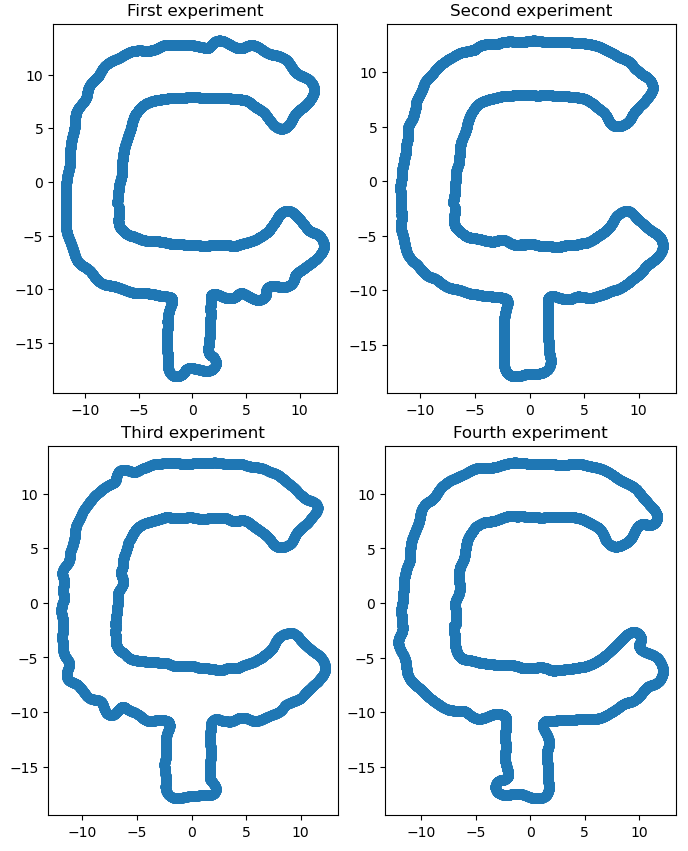
\includegraphics{images/experiments.png}}
    \caption{Path followed by the robot for each experiment.}
    \label{fig:path}
\end{figure}

Out of these experiments, the third one was the significantly faster than the other ones. This was expected since it is the one with the highest maximum linear velocity (and linear/angular acceleration). In general, by analyzing all runs, it seems that higher angular acceleration values lead to faster loop times.

Regarding stability, the second experiment's path was the one with the tightest fit. Two factors contribute to this outcome: higher angular acceleration, and lower linear velocity. In the \emph{Flatland} simulator, walls can only be vertical or horizontal lines. This leads to a \textit{jagged edge} effect on the curved parts of the map. This causes the robot to frequently attempt to set the angular velocity to high values; whenever it finds one of these edges (i.e., a corner). Higher angular accelerations provide the robot with more \textit{agility}, but this can become problematic if the maximum angular velocity is also high: it leads to instability. The low linear velocity of this experiment leads to a more stable path: less distance covered without updates from the robot's \textit{brain}.

Given that the robot only reacts to sensor's updates, to keep the path stable when the robot's maximum velocity increases, we need to increase the sensor's update frequency. This becomes evident when looking at experiments one, two, and three. Between experiment one and two, increasing the angular acceleration of the robot, increases its agility and leads to a more stable path. In experiment three, even though we increase the angular acceleration by a large amount, the increase in linear velocity leads to a significantly more unstable path. Furthermore, ``Fig.~\ref{fig:update_rate}'' shows the paths followed by the robot in experiment three with different sensor update rates: 10Hz and 100Hz. Notice that the higher update rate leads to a much more stable path, and a lower loop time (58.25 seconds vs 54.35 seconds): stable paths are shorter.

\begin{figure}[htbp]
    \centerline{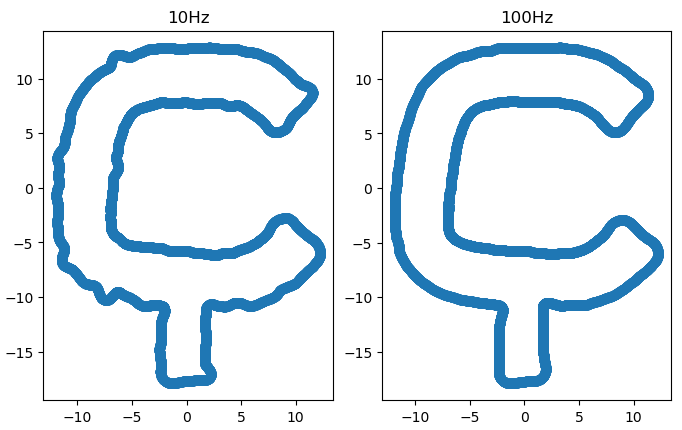
\includegraphics[width=0.8\linewidth]{images/update_rate.png}}
    \caption{Path followed by the robots with different sensor update rate.}
    \label{fig:update_rate}
\end{figure}

Experiments one and four differ only on the loop direction, i.e., which side of the robot is closest to the wall. The loop time in experiment four is about 1.35 seconds lower, which is not very significant ($\approx 1\%$ decrease). For this reason, we consider that the direction does not influence the loop time.

\section{Future work}

Although we reached the goals proposed for the project, there are still some edges that could be polished.

Firstly, as can be seen in ``Fig.~\ref{fig:path}'', there are some cases where the path of the robot is unstable, especially when looking at the curves of the letter. This is because the rate at which the robot receives the reading from the sensors is constant. This constant update rate makes it so that some corrections to the trajectory of the robot with higher angular velocity may last longer than necessary, causing the robot to turn longer than it should. To fix this, the robot should be able to estimate the shape of the wall by using the LiDAR information and adapt the angular velocity accordingly; taking into account both its current position and the estimated reachable positions for the robot upon receiving the next reading.    

On top of that, to claim the software is working as intended it still needs to be tested on a real-life robot. Simulations were the main focus of the work, with no real-life testing. Since in some cases, the simulations work differently than in real life, due to environmental characteristics or the material present in the environment, and as such, the software should be verified using a real turtle bot.

\section{Conclusions}

Even though the robot's capabilities are limited, it is possible to write algorithms such that it completes the task of following a wall and stopping at the right location.

The developed robot is able to: adapt its linear velocity to have time to react to incoming obstacles, complete loops around the whole map, distinguish between the bottom part of the cedilla and the edges of the C letter (flat surfaces), and stop at the correct location. The robot is highly configurable (explored in Sec.~\ref{sec:results}) and the given configuration can affect whether the robot is able to complete its task. The most important aspect of configuring the robot is the balance between the \textit{agility} and the \textit{speed} of the robot. Furthermore, the higher the update rate of the sensor, the more stable the path of the robot.

We believe the task of stopping at the bottom of the cedilla could have been made easier by making the edges of the "C" letter curved. This way, only the cedilla would be straight, and we wouldn't have to calculate the length of the wall.

\bibliographystyle{plain}
\bibliography{egbib}

\end{document}
